% Chapter 2

\chapter{Examples} % Chapter title

\label{ch:examples} % For referencing the chapter elsewhere, use \autoref{ch:examples} 

%----------------------------------------------------------------------------------------

\lipsum[1]

%----------------------------------------------------------------------------------------

\section{Examples}

This template for \LaTeX\ has two goals:
\begin{enumerate}
\item Provide students with an easy-to-use template for their Master's or PhD thesis (though it might also be used by other types of authors for reports, books, etc.).
\item Provide a classic, high-quality typographic style that is inspired by \citeauthor{bringhurst:2002}'s ``\emph{The Elements of Typographic Style}'' \citep{bringhurst:2002}.
\marginpar{\myTitle \myVersion}
\end{enumerate}

The \textsmaller{GNU}  a \emph{full} MiK\TeX\ or \TeX Live installation right \texttt{classicthesis}  away and, therefore, it uses only freely available fonts.


If you like the style then I would appreciate a postcard:
\begin{center}
Andre Miede \\
Detmolder Strasse 32 \\
31737 Rinteln \\
Germany
\end{center}

\noindent The postcards I received so far are available at:
\begin{center}
 \url{http://postcards.miede.de}
\end{center}

\marginpar{A well-balanced line width improves the legibility of the text. That's what typography is all about, right?} So far, many theses, some books, and several other publications have been typeset successfully with it. If you are interested in some typographic details behind it, enjoy Robert Bringhurst's wonderful book. % \citep{bringhurst:2002}.

\paragraph{Important Note:} Some things of this style might look unusual at first glance, many people feel so in the beginning. However, all things are intentionally designed to be as they are, especially these:
\begin{itemize}
\item No bold fonts are used. Italics or spaced small caps do the job quite well.
\item The size of the text body is intentionally shaped like it is. It supports both legibility and allows a reasonable amount of information to be on a page. And, no: the lines are not too short.
\item The tables intentionally do not use vertical or double rules. See the documentation for the \texttt{booktabs} package for a nice discussion of this topic.\footnote{To be found online at \\ \url{http://www.ctan.org/tex-archive/macros/latex/contrib/booktabs/}.}
\item And last but not least, to provide the reader with a way easier access to page numbers in the table of contents, the page numbers are right behind the titles. Yes, they are \emph{not} neatly aligned at the right side and they are \emph{not} connected with dots that help the eye to bridge a distance that is not necessary. If you are still not convinced: is your reader interested in the page number or does she want to sum the numbers up?
\end{itemize}

\noindent Therefore, please do not break the beauty of the style by changing these things unless you really know what you are doing! Please.

If you want to use backreferences from your citations to the pages they were cited on, change the following line from:
\begin{lstlisting}[breaklines=false,frame=lt]
\setboolean{enable-backrefs}{false}
\end{lstlisting}
to
\begin{lstlisting}[breaklines=false,frame=lt]
\setboolean{enable-backrefs}{true}
\end{lstlisting}

\begin{verbatim}
\usepackage[spanish,es-lcroman]{babel}
\end{verbatim}


\section{A New Section}

\lipsum[2]

Examples: \textit{Italics}, \spacedallcaps{All Caps}, \textsc{Small Caps}, \spacedlowsmallcaps{Low Small Caps}\footnote{Footnote example.}.

%------------------------------------------------

\subsection{Test for a Subsection}

\graffito{Note: The content of this chapter is just some dummy text.}
\lipsum[3-5]

%------------------------------------------------

\subsection{Autem Timeam}

\lipsum[6]

%----------------------------------------------------------------------------------------

\section{Another Section in This Chapter}

\lipsum[7]

Sia ma sine svedese americas. Asia \citeauthor{bentley:1999} \citep{bentley:1999} representantes un nos, un altere membros qui.\footnote{De web nostre historia angloromanic.} Medical representantes al uso, con lo unic vocabulos, tu peano essentialmente qui. Lo malo laborava anteriormente uso.

\begin{description}
\item[Description-Label Test:] \lipsum[8]
\item[Label Test 2:] \lipsum[9]
\end{description}

\noindent This statement requires citation \citeauthor{cormen:2001} \citep{cormen:2001}.

%------------------------------------------------

\subsection{Personas Initialmente}

\lipsum[10]

\subsubsection{A Subsubsection}
\lipsum[11]

\paragraph{A Paragraph Example} \lipsum[12]

\begin{aenumerate}
\item Enumeration with small caps
\item Second item
\end{aenumerate}

\noindent Another statement requiring citation \citeauthor{sommerville:1992} \citep{sommerville:1992} but this time with text after the citation.

\begin{table}
\myfloatalign
\begin{tabularx}{\textwidth}{Xll} \toprule
\tableheadline{labitur bonorum pri no} & \tableheadline{que vista}
& \tableheadline{human} \\ \midrule
fastidii ea ius & germano &  demonstratea \\
suscipit instructior & titulo & personas \\
\midrule
quaestio philosophia & facto & demonstrated \citeauthor{knuth:1976} \\
\bottomrule
\end{tabularx}
\caption[Autem timeam deleniti usu id]{Autem timeam deleniti usu id. \citeauthor{knuth:1976}}  
\label{tab:example}
\end{table}

\enlargethispage{2cm}

%------------------------------------------------

\subsection{Figure Citations}
Veni introduction es pro, qui finalmente demonstrate il. E tamben anglese programma uno. Sed le debitas demonstrate. Non russo existe o, facite linguistic registrate se nos. Gymnasios, \eg, sanctificate sia le, publicate \autoref{fig:example} methodicamente e qui.

Lo sed apprende instruite. Que altere responder su, pan ma, \ie, signo studio. \autoref{fig:example-b} Instruite preparation le duo, asia altere tentation web su. Via unic facto rapide de, iste questiones methodicamente o uno, nos al.

\begin{figure}[bth]
\myfloatalign
\subfloat[Asia personas duo.]
{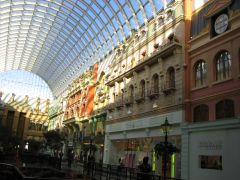
\includegraphics[width=.45\linewidth]{gfx/example_1}} \quad
\subfloat[Pan ma signo.]
{\label{fig:example-b}
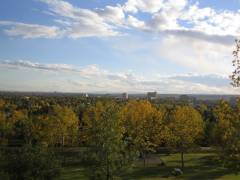
\includegraphics[width=.45\linewidth]{gfx/example_2}} \\
\subfloat[Methodicamente o uno.]
{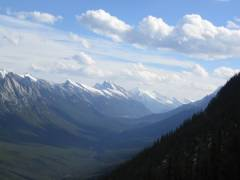
\includegraphics[width=.45\linewidth]{gfx/example_3}} \quad
\subfloat[Titulo debitas.]
{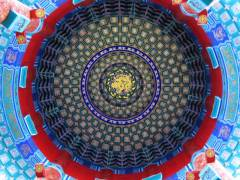
\includegraphics[width=.45\linewidth]{gfx/example_4}}
\caption[Tu duo titulo debitas latente]{Tu duo titulo debitas latente.}\label{fig:example}
\end{figure}

\section{Some Formulas}

Due to the statistical nature of ionisation energy loss, large fluctuations can occur in the amount of energy deposited by a particle traversing an absorber element\footnote{Examples taken from Walter Schmidt's great gallery: \\ \url{http://home.vrweb.de/~was/mathfonts.html}}.  Continuous processes such as multiple scattering and energy loss play a relevant role in the longitudinal and lateral development of electromagnetic and hadronic showers, and in the case of sampling calorimeters the measured resolution can be significantly affected by such fluctuations in their active layers.  The description of ionisation fluctuations is characterised by the significance parameter $\kappa$, which is proportional to the ratio of mean energy loss to the maximum allowed energy transfer in a single collision with an atomic electron: \graffito{You might get unexpected results using math in chapter or section heads. Consider the \texttt{pdfspacing} option.}
\begin{equation}
\kappa =\frac{\xi}{E_{\mathrm{max}}} %\mathbb{ZNR}
\end{equation}
$E_{\mathrm{max}}$ is the maximum transferable energy in a single collision with an atomic electron.
\[E_{\mathrm{max}} =\frac{2 m_{\mathrm{e}} \beta^2\gamma^2 }{1 + 2\gamma m_{\mathrm{e}}/m_{\mathrm{x}} + \left ( m_{\mathrm{e}} /m_{\mathrm{x}}\right)^2}\ ,\]
where $\gamma = E/m_{\mathrm{x}}$, $E$ is energy and $m_{\mathrm{x}}$ the mass of the incident particle, $\beta^2 = 1 - 1/\gamma^2$ and $m_{\mathrm{e}}$ is the electron mass. $\xi$ comes from the Rutherford scattering cross section and is defined as:
\begin{eqnarray*} \xi  = \frac{2\pi z^2 e^4 N_{\mathrm{Av}} Z \rho
\delta x}{m_{\mathrm{e}} \beta^2 c^2 A} =  153.4 \frac{z^2}{\beta^2}
\frac{Z}{A}
\rho \delta x \quad\mathrm{keV},
\end{eqnarray*}
where

\begin{tabular}{ll}
$z$ & charge of the incident particle \\
$N_{\mathrm{Av}}$ & Avogadro's number \\
$Z$ & atomic number of the material \\
$A$ & atomic weight of the material \\
$\rho$ & density \\
$ \delta x$ & thickness of the material \\
\end{tabular}

$\kappa$ measures the contribution of the collisions with energy transfer close to $E_{\mathrm{max}}$.  For a given absorber, $\kappa$ tends towards large values if $\delta x$ is large and/or if $\beta$ is small.  Likewise, $\kappa$ tends towards zero if $\delta x $ is small and/or if $\beta$ approaches $1$.

The value of $\kappa$ distinguishes two regimes which occur in the description of ionisation fluctuations:

\begin{enumerate}
\item A large number of collisions involving the loss of all or most of the incident particle energy during the traversal of an absorber.

As the total energy transfer is composed of a multitude of small energy losses, we can apply the central limit theorem and describe the fluctuations by a Gaussian distribution. This case is applicable to non-relativistic particles and is described by the inequality $\kappa > 10 $ (\ie, when the mean energy loss in the absorber is greater than the maximum energy transfer in a single collision).

\item Particles traversing thin counters and incident electrons under any conditions.

The relevant inequalities and distributions are $ 0.01 < \kappa < 10 $, Vavilov distribution, and $\kappa < 0.01 $, Landau distribution.
\end{enumerate}

%----------------------------------------------------------------------------------------

\section{Various Mathematical Examples}

If $n > 2$, the identity \[t[u_1,\dots,u_n] = t\bigl[t[u_1,\dots,u_{n_1}], t[u_2,\dots,u_n] \bigr]\] defines $t[u_1,\dots,u_n]$ recursively, and it can be shown that the alternative definition \[t[u_1,\dots,u_n] = t\bigl[t[u_1,u_2],\dots,t[u_{n-1},u_n]\bigr]\] gives the same result.